%&pdflatex
\documentclass{standalone}
\usepackage{tikz}
\usetikzlibrary{arrows}
\usetikzlibrary{shapes}
\usetikzlibrary{positioning}
\usetikzlibrary{snakes}

\begin{document}

\begin{tikzpicture}
\node[inner sep=0pt] (three1) at (-2,0) {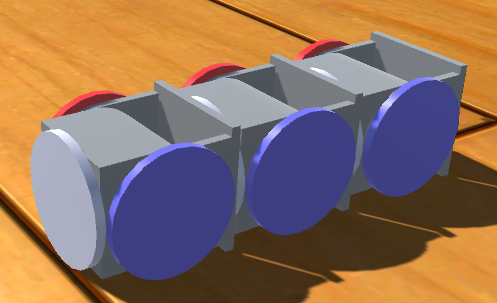
\includegraphics[width=2cm]{../library/unity/threeModules.png}};
\node[inner sep=0pt] (three2) at (2,0) {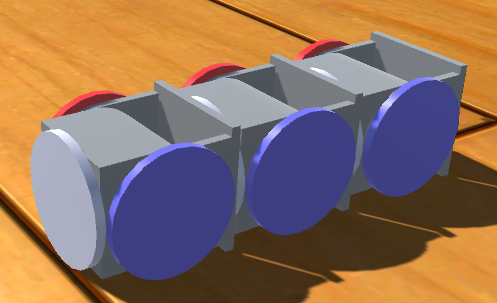
\includegraphics[width=2cm]{../library/unity/threeModules.png}};
\node[inner sep=0pt] (body) at (0,-2) {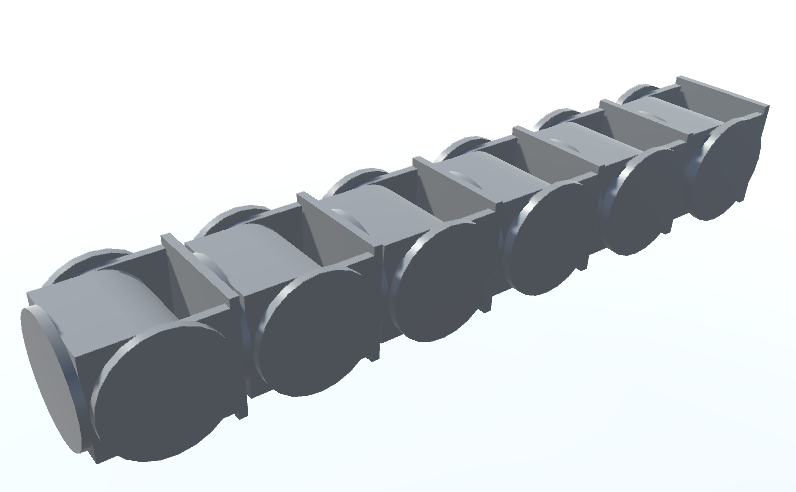
\includegraphics[width=4cm]{../library/unity/body.png}};

\draw[->,ultra thick] ([xshift=-0.3cm]three1.east) -|  ([yshift=0.5cm]body.north) -- (body);
\draw[->,ultra thick] ([xshift=0.3cm]three2.west) -|  ([yshift=0.5cm]body.north) -- (body);
\end{tikzpicture}

\end{document}



